\documentclass[11pt]{article}
\usepackage[top=1.0in, bottom=1.0in, left=1.0in, right=1.0in]{geometry}
\usepackage{Sweave}
\renewcommand{\baselinestretch}{1.2}
\usepackage{graphicx}
\usepackage{hyperref}
\usepackage{natbib}
\bibliographystyle{besjournals} 
\usepackage{amsmath}
\newcommand{\R}[1]{\label{#1}\linelabel{#1}}
\usepackage{gensymb}
\usepackage{lineno}
\usepackage{caption}

\renewcommand{\thetable}{S\arabic{table}}
\renewcommand{\thefigure}{S\arabic{figure}}

\captionsetup{font={sf,small}} 


\begin{document}

\setkeys{Gin}{width=0.95\textwidth}

% \linenumbers

\title{Biological and climatic constraints drive reproductive synchrony\\\emph{Supplementary figures}}

% \date{\today}
\author{Victor, Mike, Lizzie}
\maketitle
  
% \noindent $^{1}$Forest and Conservation Sciences, University of British Columbia, Vancouver, BC, Canada\\



\begin{figure}[htbp]
  \centering
  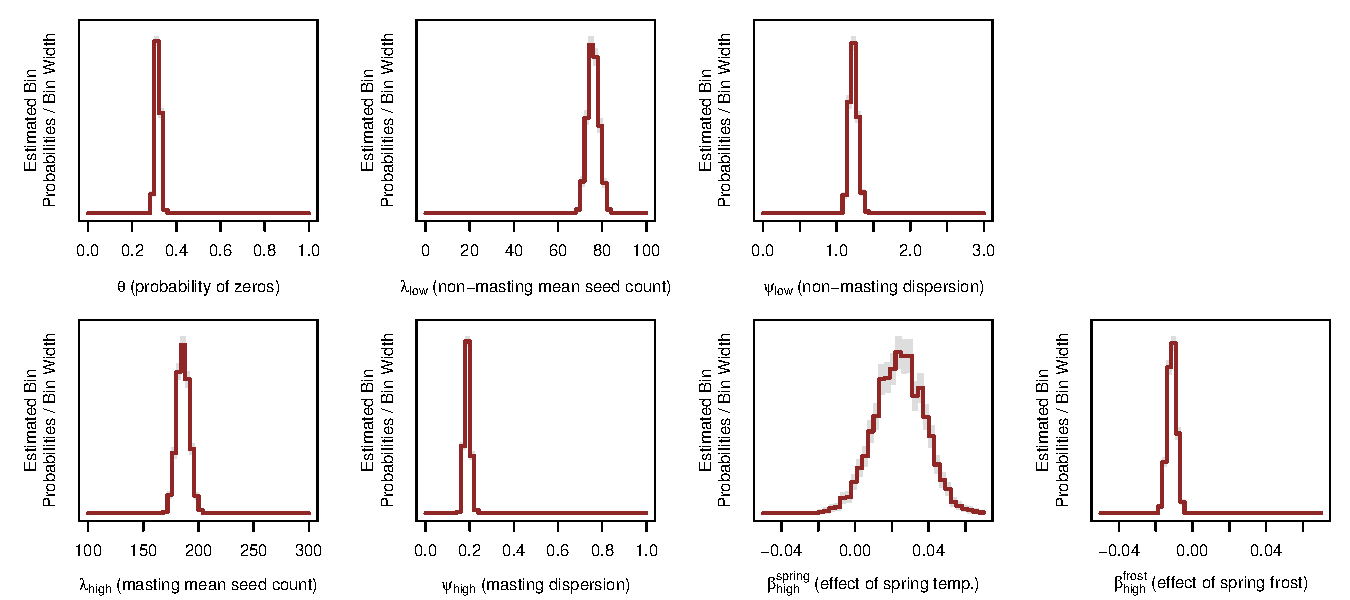
\includegraphics{figures/new/supp/negbin_parameters.pdf}
  \caption{\textbf{Posterior distributions of the parameters related to seed count distributions (main text model).} These parameters control the number of seeds produced in low and high states. \emph{Spring temp.} corresponds to the average spring temperature in April and May. \emph{Spring frost} correspond to the growing degree days accumulated until the last frost day. See Methods for details. }
  \label{fig:seedcount}
\end{figure}

\begin{figure}[htbp]
  \centering
  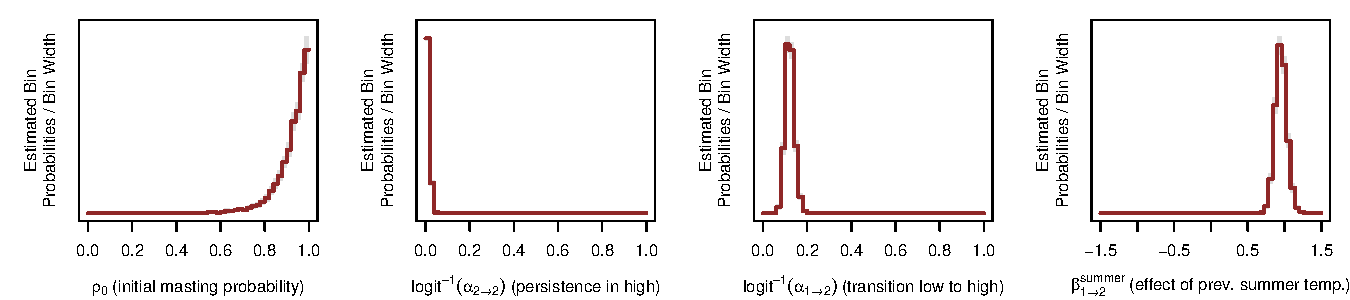
\includegraphics{figures/new/supp/transition_parameters.pdf}
  \caption{\textbf{Posterior distributions of the parameters related to state transitions (main text model).} These parameters control the transition probabilities between states (1 = low, 2 = high). \emph{Prev. summer temp.} corresponds to the average maximum temperature in July and August (of the previous year). See Methods for details. }
  \label{fig:transition}
\end{figure}

\begin{figure}[htbp]
  \centering
  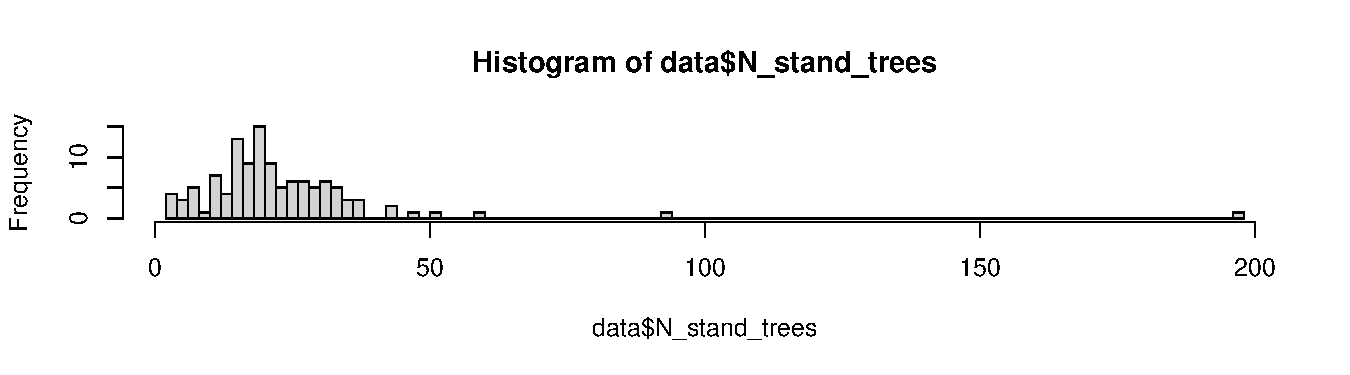
\includegraphics{figures/new/supp/coldvswarmsummer.pdf}
  \caption{\textbf{Posterior distributions of transition probability from low to high reproductive states in a cold vs. a warm summer.} On average, the transition probability during a warm summer is 3.6 times higher than during a cold summer.}
  \label{fig:coldvswarm}
\end{figure}


\begin{figure}[htbp]
  \centering
  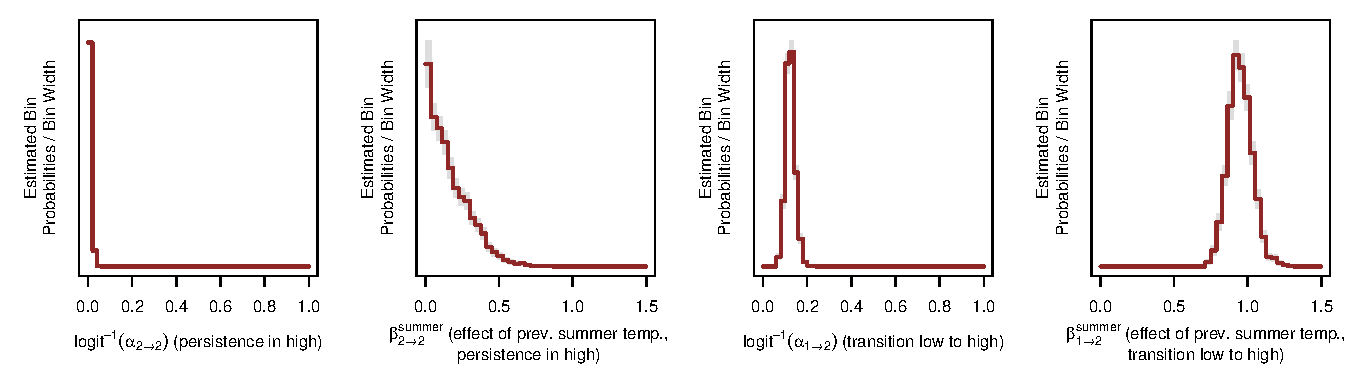
\includegraphics{figures/new/supp/transition_parameters_fullsummer.pdf}
  \caption{\textbf{Posterior distributions of the parameters related to state transitions (model with summer temp. on both transitions).} In this model, we tested whether the persistence in a high state was affected by previous summer temperature ($\beta^\text{summer}_{2 \rightarrow 2}$). Because this model is more complex (one additional parameter), we constrained both beta parameters to be > 0. This lower bound constraint limits the effect of higher summer temperatures (both previous and current year) to increase seed count as is widely expected (though this constraint was not present in the model presented in the main text and we found the same positive response).}
  \label{fig:transitionboth}
\end{figure}

\begin{figure}[htbp]
  \centering
  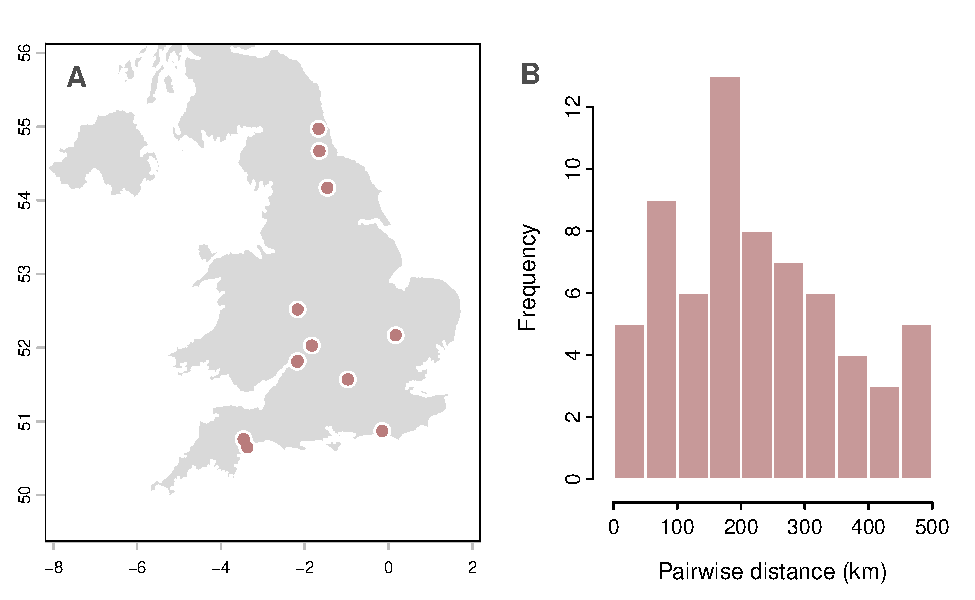
\includegraphics{figures/new/supp/map.pdf}
  \caption{\textbf{(A) Map of the beech forest sites (England).} We used data from 171 trees on 12 sites. \\
  \textbf{(B) Distributions of pairwise distance between sites.} Sites are on average 224 km apart.}
  \label{fig:map}
\end{figure}

\begin{figure}[htbp]
  \centering
  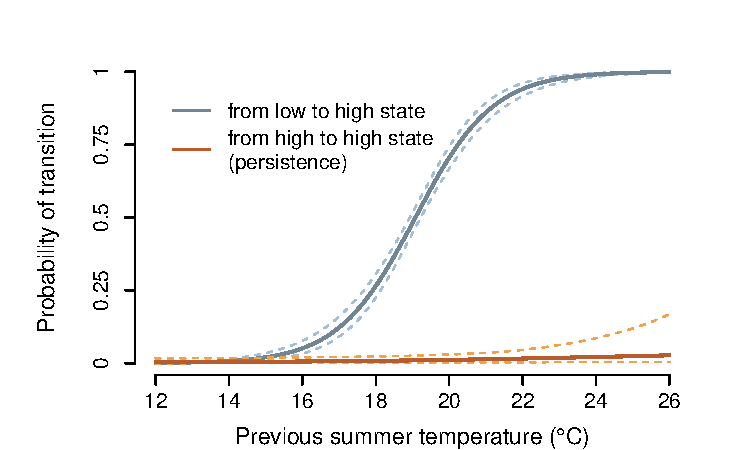
\includegraphics[width=0.6\linewidth]{figures/new/supp/summertempdepend.pdf}
  \caption{\textbf{Effect on previous summer temperature on the probability of transition from a low reproductive to a high reproductive state, and on the probability of persistence in a high reproductive state (model with summer temp.
on both transitions, see Supp. Fig \ref{fig:transitionboth}).} Even when summer temperature could influence both the transition to a high state and the persistence in a high state, trees could not become stuck indefinitely in a high state.}
  \label{fig:warmpersist}
\end{figure}



\end{document}
